
\label{capitolo1}\chapter{Introduzione}


\section{Introduzione}

boh..


\section{Animazione e Simulazione}

A partire dagli anni '80, lo sviluppo animazioni per la visualizzazione
di algoritmi stata in continuo aumento. La prima testimonianza che
si ha {}``Sorting out sorting'' \cite{video}, un video di presentazione
degli algoritmi di ordinamento, primo nel suo genere.

Dal 1981 fino ad oggi, le rappresentazioni di algoritmi e strutture
dati si sono diffuse ed hanno trovato il loro scopo finale come supporto
per studenti ed insegnanti nei relativi corsi universitari.

Osservando il materiale disponibile ad oggi sul web e come ci fa notare
\cite{MatrixPro}, possiamo riconoscere che esistono principalmente
due forme in cui si sono sviluppati i tool di algorithm visualization:
l'animazione e la simulazione.

La prima consiste in una visualizzazione degli effetti che un algoritmo
predefinito ha su una struttura dati definita dal programmatore. L'utente,
in questo caso, assiste passivamente all'animazione osservandone i
risultati sulla struttura dati.

Nel secondo caso parliamo di simulazione in quanto l'utente manipola
gli oggetti messi a disposizione dal programmatore secondo le modifiche
permesse dalla struttura in modo da creare una sequenza di passi analoghi
a quelli dell'algoritmo che si sta analizzando.

Naturalmente questa una classificazione grossolana, in quanto ogni
tool ha le sue particolari caratteristiche. Le funzionalit introdotte
negli anni nelle varie applicazioni disponibili hanno permesso una
seconda classificazione pi accurata in base all'interazione che tali
visualizzazioni hanno con gli studenti. Il risultato di gruppo di
lavoro su {}``Improving the Educational Impact of Algorithm Visualization''
(Giugno 2002, ITiCSE, Denmark) stata la suddivisione in 6 categorie
delle varie forme di insegnamento in base al supporto di visualizzazione
utilizzato, riportata in \cite{AV-compare}: 
\begin{enumerate}
\item No viewing (come lo traduco??), gli studenti non hanno a disposizione
nessun supporto visivo, (o al massimo immagini non animate);proprio 
\item Viewing, osservazione passiva dell'esecuzione dell'algoritmo, in cui
possibile al massimo controllare il flusso di esecuzione tramite comandi
di undo - redo - rewind.... 
\item Responding, come per viewing consiste nell'osservazione della rappresentazione
dell'algoritmo, durante la quale allo studente richiesto di rispondere
ad una serie di domande, o svolgere esercizi su carta, relativi all'argomento
presentato. 
\item Changing, modificare la visualizzazione principalmente attraverso
la personalizzazione dei dati in ingresso all'algoritmo, in modo da
analizzare il comportamento dell'algoritmo nei vari casi. 
\item Constructing, costruire la propria visualizzazione dell'algoritmo
che si sta studiando 
\item Presenting, presentare ad un pubblico la visualizzazione di un particolare
algoritmo, per poi procedere ad una discussione sull'argomento. 
\end{enumerate}
I risultati delle tipologie di insegnamento appena riportate sono
soggetto di numerosi studi presenti e passati, e una sinteri dei risulati
raccolti presente nella \ref{sec:studi-effettuati-sull'efficacia}


\section{\label{sec:studi-effettuati-sull'efficacia}Studi effettuati sull'efficacia
degli AV nell'insegnamento}

A seguito della classificazione delle tipologie di insegnamento dei
corsi riguardanti Algoritmi e Strutture Dati, e la loro interazione
con le tecnologie di visualizzazione algoritmi, sono stati effettuati
numerosi studi a proposito dell'efficacia dell'introduzione di queste
nuove tecniche sull'apprendimento degli studenti.

Un'analisi generale riportata in \cite{AV-compare}. Lo studio \cite{byrne}
hanno riportato gli studenti analizzati che hanno utilizzato un supporto
alle lezioni di tipo 3(responding) e 5(construction), hanno ottenuto
risultati migliori nei test, rispetto ad altri studenti che non ne
avevano fatto uso, o che avevano utilizzato una semplice animazione
(livello 2). Nello studio \cite{jarc} sono stati raccolti invece
risultati in conflitto con i primi. Secondo quest'ultimo, non c'
stata nessuna differenza significati nei risultati ottenuti dagli
studenti con l'una o l'altra tipologia di supporto alle lezioni.

Lo studio riportato in \cite{AV-compare} mette in risalto il miglioramento
degli studenti, a seconda della tecnica di supporto visivo utilizzata,
tenendo anche conto anche delle conoscenze precedenti dei soggetti.
Gli studenti, provenienti da 3 diverse universit, sono stati soggetti
di un pre-test, nel quale venivano valutate le loro conoscenze e attitudini,
prima delle lezioni. A seconda dei risultati, sono stati divisi in
tre gruppi per ognuno dei quali sono state effettuate una serie di
lezioni sull'argomento degli algoritmi di ordinamento con l'utilizzo
di 3 diverse tecniche: 
\begin{enumerate}
\item Lezioni frontali senza supporti visivi 
\item Lezioni frontali con l'utilizzo da parte del docente di una presentazione
e di un tool di visualizzazione di algoritmi 
\item Lezioni frontali (come gruppo 2) con l'aggiunta di ore supplementari
di attivit di laboratorio, in cui gli studenti potevano utilizzare
singolarmente un'applicazione (JHAVE' \cite{JHAVE}) che permette
di osservare l'animazione degli algoritmi integrata con domande ad-hoc. 
\end{enumerate}
A seguito di queste attivit, gli studenti sono stati esaminati con
un test uguale per tutti.

I risultati ottenuti si sono rilevati concordi con \cite{byrne} in
quanto rapportando le conoscenze iniziali degli studenti con gli esiti
dei test di verifica, si osservato che maggiore l'interazione con
lo strumento di supporto, maggiori sono i progressi ottenuti dagli
studenti.

A seguito di questo studio si quindi potuto supporre che i risultati
non significativi di \cite{jarc} fossero dovuti ad un'inadeguata
tecnica di raccolta: nel caso delle domande gli studenti, lasciati
liberi a se stessi e non confinati in un laboratorio, hanno affrontato
il tool come un gioco e non come uno strumento educativo.

Per quanto riguarda la categoria di applicazioni 6 (presentig), purtroppo
non sono ancora presenti studi che indichino l'efficacia di tale tecnica
di insegnamento.

{[}Aggiungere testimonianza corso di studi algoritmie strutture dati
in cui sono state adoperate le tecniche sopra, obbligando gli studenti,
che le hanno trovate utili e il 65\% ha passato l'esame al primo colpo{]}


\section{Come creare un buon AV}

Algoviz \cite{wikiAlgoViz} costituisce il sito di riferimento per
studenti docenti e chiunque altro sia interessato nella ricerca di
un'applicazione che raccolga visualizzazioni di algoritmi, o l'animazione
di una particolare struttura. Dal 2006 il sito raccoglie in un proprio
archivio (continuamente aggiornato) tutte gli strumenti rintracciabili
sul web relativi a questo argomento. Tale sito stato anche il punto
di partenza di questa tesi, in quanto ha permesso di esplorare e analizzare
i principali toolkit per sviluppatori presenti al momento, e inoltre
contiene un'interessante guida per chi si appresta a realizzare una
propria visualizzazione di algoritmi.

Si riporta ora una sintesi dei principi chiave esposti nella guida: 
\begin{description}
\item [{{Coinvolgere}}] fare in modo che l'utente partecipi attivamente
durante l'animazione dell'algoritmo, evitando le presentazioni statiche
e passive 
\item [{{Semplificare}}] ridurre la complessit dell'applicazione, a partire
dall'interfaccia grafica. Per quanto riguarda l'esposizione dei concetti,
nascondere per quanto possibile i dettagli implementativi degli algoritmi,
e animare le i singoli passi operazioni pi complesse. L'applicazione
inoltre deve essere talmente semplice da necessitare di una minima
documentazione relativa al proprio funzionamento, in quanto l'utente
deve riuscire ad avviarla e comprenderne l'utilizzo fin dal primo
avvio. 
\item [{{DataSet}}] fornire diverse tipologie di gestione dei dati in
ingresso

\begin{itemize}
\item Dati inseriti dall'utente, per permettere l'eplorazione di tutte le
possibili configurazioni, dando la possibilit allo studente di verificare
il comportamento della struttura in casi particolari da lui costruiti; 
\item Dati random, di cui l'utente potrebbe controllare solo alcuni parametri
(con la dimensione, il range, ecc..); 
\item Dati pre-costruiti ad hoc, che permettano allo studente di analizzare
il comportamento chiave dell'algortimo in situazioni chiave, preparate
ad hoc dal docente o dal programmatore. Questa funzionalit risulta
utile perch generalmente gli studenti (soprattutto se alle prime armi)
non ha la fantasia necessaria per creare casi particolari di testing. 
\end{itemize}
\item [{{Controllo}}] se si tratta di una semplice rappresentazione animata
dell'esecuzione di un programma su di una struttura dati, fondamentale
permettere allo studente di controllare il flusso dell'animazione
attraverso una serie di comandi, quali il controllo della velocit
(nel caso si parli di un'animazione continua), possibilit di procedere
passo-passo, andare avanti e indietro nell'animazione. Algoviz riporta
che l'utilizzo dell'animazione spezzata in passi, produce risultati
migliori nell'apprendimento rispetto ad una visualizzazione continua
del funzionamento. 
\end{description}

\section{\label{sec:Strumenti-Disponibili}Strumenti Disponibili}

La relazione \cite{AlgoViz} redatta dal gruppo di lavoro di Algoviz,
illustra il lavoro di raccolta di AV da essi realizzato nel 2006:
sono stati trovati circa 350 AV all'epoca, che sono quindi stati raccolti
e classificati nel catalogo presente nel sito, il quale settimanalmente
aggiornato e ad oggi contiene pi di 500 visualizzazioni. Gran parte
degli strumentu catalogati riguarda gli argomenti principali dell'insegnamento
di Algoritmi e Strutture dati, primo fra tutti il problema dell'ordinamento,
al quale seguono le strutture di ricerca (ABR) strutture lineari e
gli algoritmi sui grafi.

A partire da questa raccolta, si sono analizzati i principali pacchetti
che potenzialmente costituivano un punto di partenza per altri sviluppatori
dal quale partire per creare la propria applicazione di animazione
di algoritmi. Gran parte delle applicazioni raccolte consistono in
passive rappresentazioni di algortimi che agiscono su strutture dati
preinstallate (quindi non personalizzabili) nelle quali l'utente coinvolto
solo per quanto riguarda il controllo del flusso. Esistono per alcune
eccezioni, in cui tale rappresentazione arricchita con funzionalit
interessanti che catturano e focalizzano meglio l'attenzione dello
studente sull'argomento.

Di seguito sono descritti alcuni dei principali pacchetti che sono
stati analizzati durante la ricerca. Molti altri software sono stati
esaminati, ma in questa circostanza non vengono riportati, in quanto
sono risultati presentare caratteristiche molto simili a quelle dei
programmi che ora verranno esposti. 
\begin{description}
\item [{{Animal}}] Il software Animal \cite{Animal} fornisce 
\item [{{JHAVE'}}] pacchetto migliore, classificato al 2 posto, in quanto
non si capice come modificarlo e le domande fanno cagare 
\item [{{MatrixPro}}] e Trackla2, vedi seguito 
\end{description}
\begin{figure}[htbp]
\centering
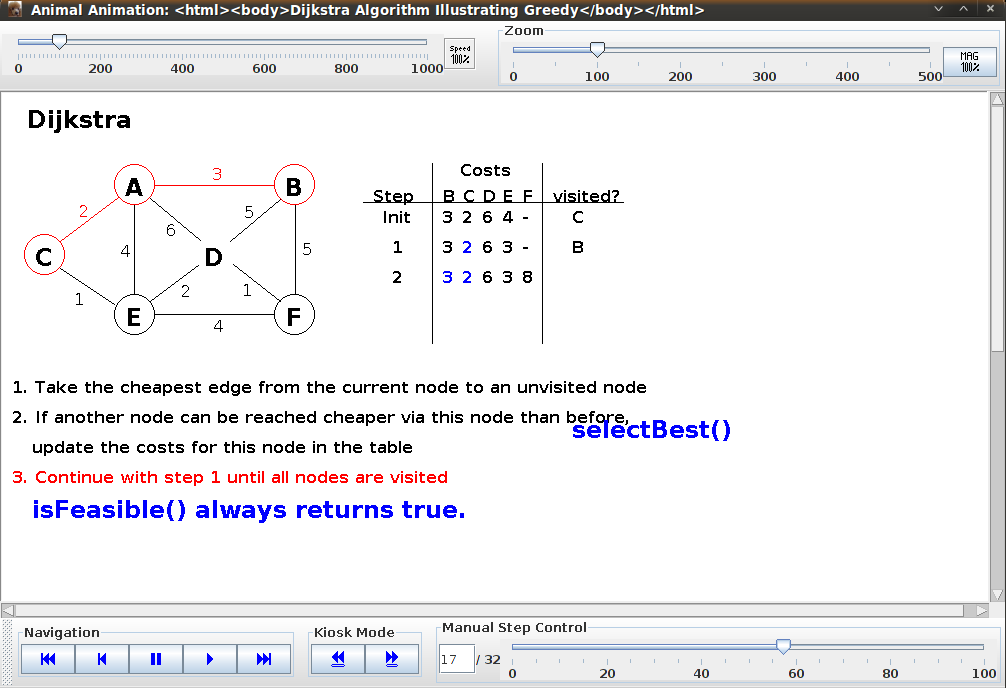
\includegraphics[scale=0.25]{images/Animal_screenshot.png}
\caption{Screenshot di Animal}
\end {figure}

\begin{figure}
\centering
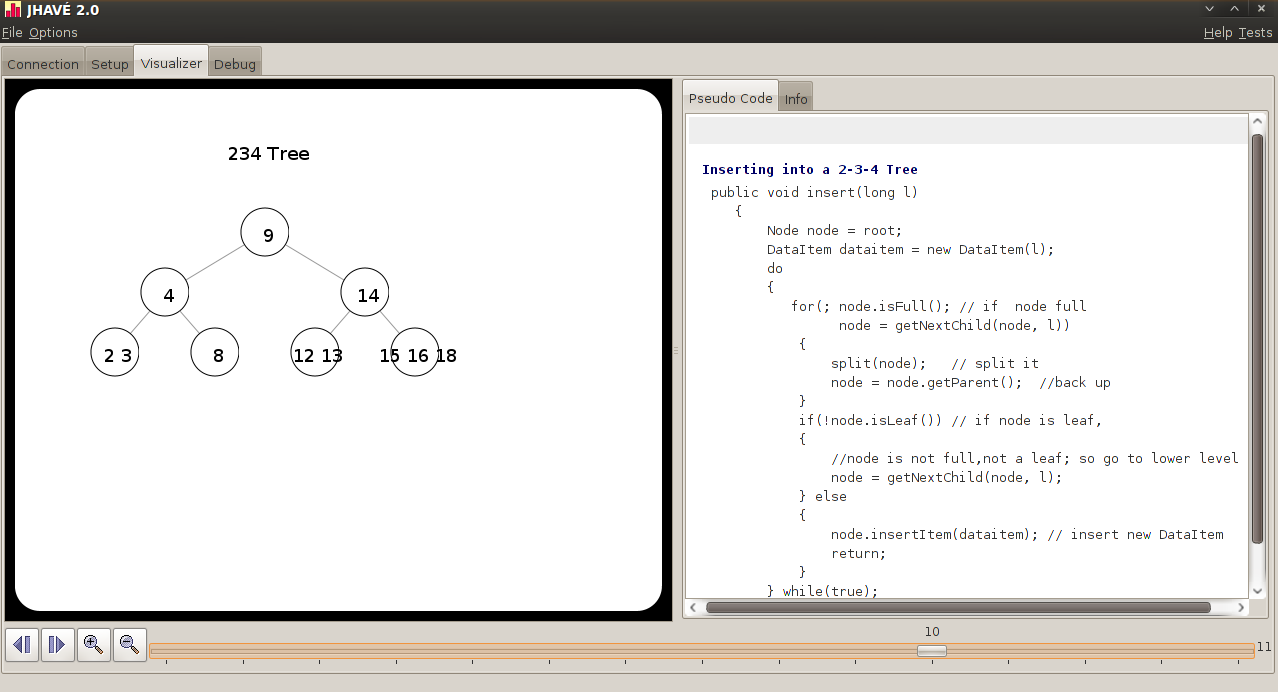
\includegraphics[scale=0.25]{images/JHAVE_screenshot.png}
\caption{Screenshot di JHAVE}
\end{figure}

\begin{figure}
\centering
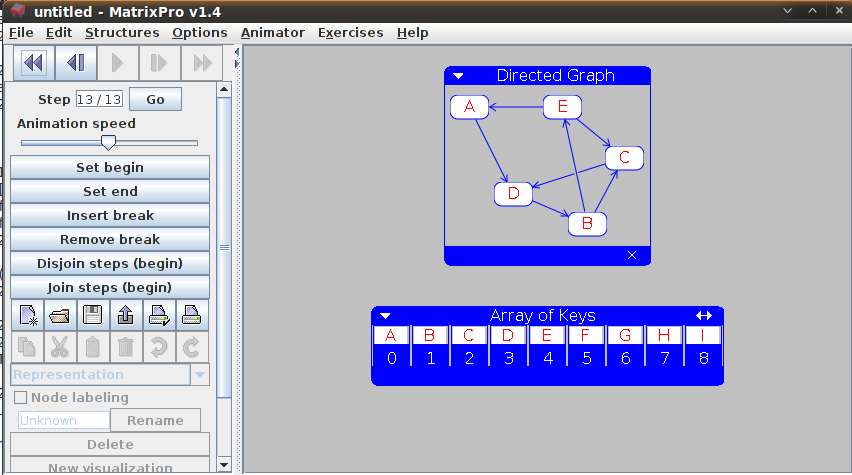
\includegraphics[scale=0.25]{images/MatrixPro_screenshot.png}
\caption{Screenshot di MatrixPro}
\end{figure} 

